\documentclass[a4paper,12pt]{jarticle}
\usepackage[dvipdfmx]{graphicx}
\usepackage{amsmath}
\usepackage{subfigure}
\usepackage{comment}

\setlength{\hoffset}{0cm}
\setlength{\oddsidemargin}{-3mm}
\setlength{\evensidemargin}{-3cm}
\setlength{\marginparsep}{0cm}
\setlength{\marginparwidth}{0cm}
\setlength{\textheight}{24.7cm}
\setlength{\textwidth}{17cm}
\setlength{\topmargin}{-45pt}

\renewcommand{\baselinestretch}{1.6}
\renewcommand{\floatpagefraction}{1}
\renewcommand{\topfraction}{1}
\renewcommand{\bottomfraction}{1}
\renewcommand{\textfraction}{0}
\renewcommand{\labelenumi}{(\arabic{enumi})}
%\renewcommand{\figurename}{Fig.} %図をFig.にする


%図のキャプションからコロン:を消す
\makeatletter
\long\def\@makecaption#1#2{% #1=図表番号、#2=キャプション本文
\sbox\@tempboxa{#1. #2}
\ifdim \wd\@tempboxa >\hsize
#1 #2\par 
\else
\hb@xt@\hsize{\hfil\box\@tempboxa\hfil}
\fi}
\makeatother
% 


\title{電機システム制御特論 \\
Assignment (2016/05/13)\\
}
\author{\vspace{40mm}\\
九州工業大学大学院 \hspace{0mm} 工学府\\
機械知能工学専攻\ \hspace{0mm} 知能制御工学コース \\
\vspace{5mm}\\
所属:\ 西田研究室\\
学籍番号:\ 16344217\\
提出者氏名:\ 津上 \hspace{0mm} 祐典\\\vspace{5mm}\\ }
\date{平成28年\ 5月\ 20日}

\begin{document}

%表紙
\titlepage
\maketitle
\thispagestyle{empty}

\newpage

\thispagestyle{empty}
\tableofcontents

\newpage
\setcounter{page}{1}
%%%%%%%%%%%%%%%%%%%%%%%%
\section{問題}
%%%%%%%%%%%%%%%%%%%%%%%%
DCモータの速度制御系を設計し,4象限運転を実行せよ.ただし,DCモータのパ
ラメータを表\ref{table:DC_dim}に示す.
%
\begin{table}[h]
 \centering
 \caption{DCモータのパラメータ}
 \label{table:DC_dim}
 \begin{tabular}{c|c|c} \hline
  名称 [単位]                    & 記号  & 数値\\\hline
  定格電力 [kW]                  &$P$    &150  \\\hline
  定格電圧 [V]                   &$V$    &450  \\\hline
  電機子抵抗 [$\Omega$]          &$R_a$  & 0.15 \\\hline
  電機子インダクタンス [H]        &$L_a$   &0.003\\\hline
  慣性モーメント [kg$\rm {m^3}$] &$J$     &150  \\\hline
  誘起電圧定数 [V$\cdot$s/rad]    &$K_E$   &8.50 \\\hline
  基底速度 [rpm]                &$\omega$&500  \\\hline
 \end{tabular}
\end{table}
%
%%%%%%%%%%%%%%%%%%%%%%%%%
\section{DCモータの特性}
%%%%%%%%%%%%%%%%%%%%%%%%%
はじめに,本レポートで用いるDCモータのブロック線図を図\ref{fig:DC_model}に示す.
%
\begin{figure}[bp]
 \begin{center}
  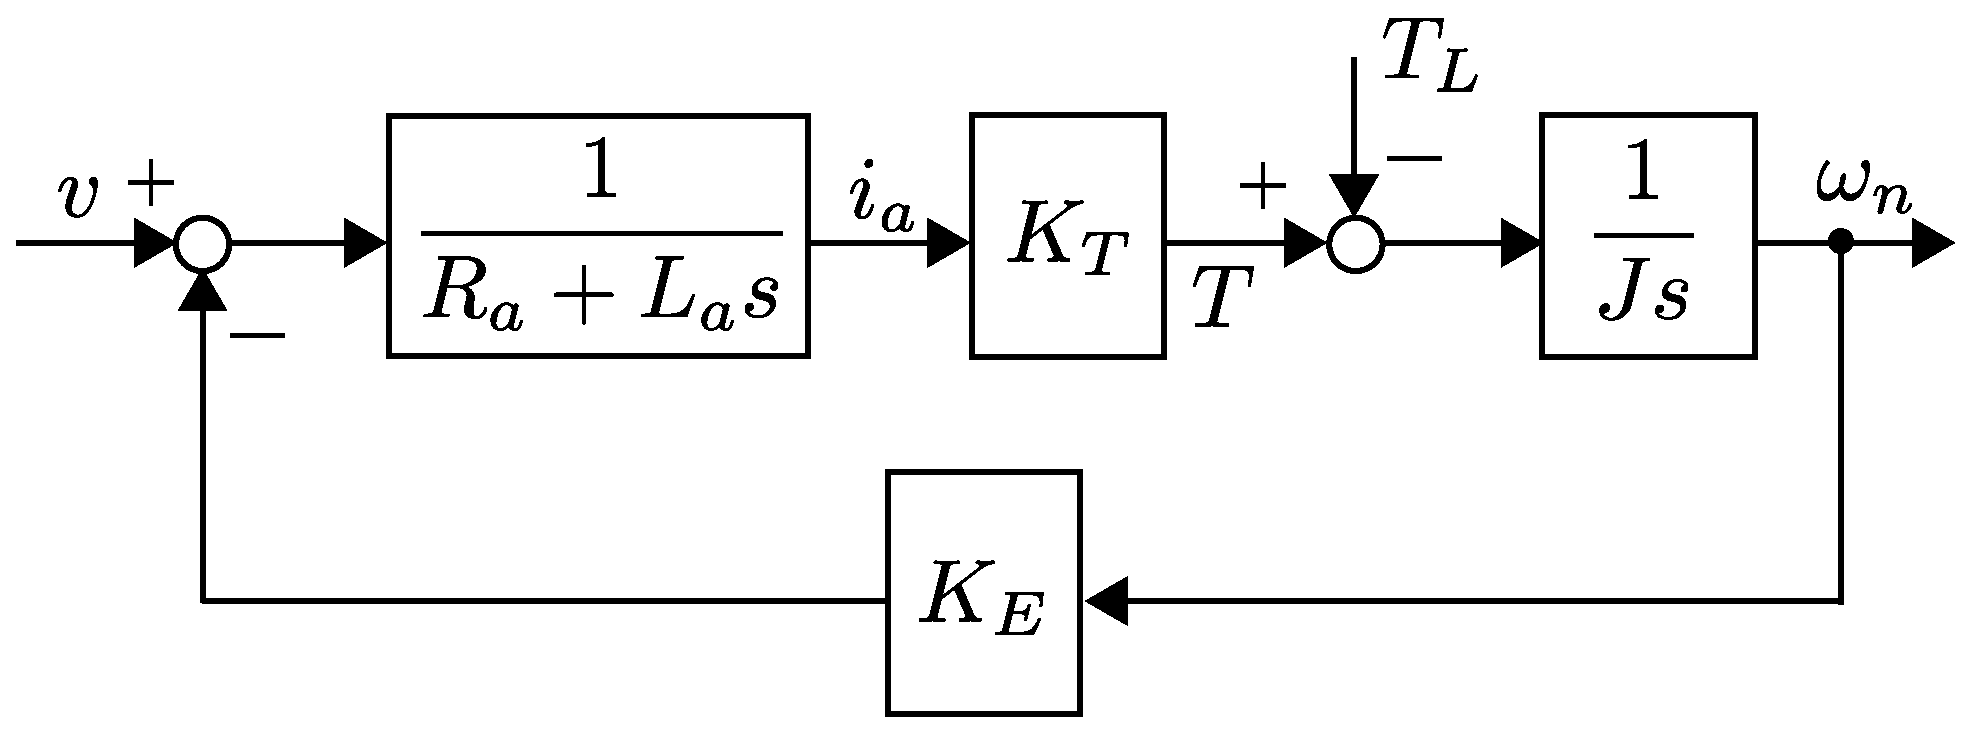
\includegraphics[width = 150mm]{fig/DC_model.eps}
 \end{center}
 \caption{DCモータのブロック線図}
 \label{fig:DC_model}
\end{figure}
%
\newpage
%
はじめに,図\ref{fig:DC_model}に示すDCモータのモデルの伝達特性を導出する.
図\ref{fig:DC_model}より
%
\begin{equation}
 \Omega_m(s)=\frac{1}{Js}\left\{\frac{K_T}{R_{a}+L_{a}s}(V-K_E\Omega_m)-T_L\right\}
\end{equation}
と表され,式変形すると,
\begin{equation*}
 \left(Js+\frac{K_{T}K_{E}}{R_{a}+L_{a}}s\right)\Omega_m(s)=\frac{K_{T}}{R_{a}+L_{a}s}-T_L
\end{equation*}
%
\begin{equation*}
 \Omega_m(s)=\frac{K_T}{JL_{a}s^2+JR_{a}s+K_TK_E}-\frac{R_{a}+L_{a}s}{JL_{a}s^2+JR_{a}s+K_TK_E}T_L
\end{equation*}
%
\begin{equation}
 \Omega_m(s)=\frac{\frac{1}{K_E}}{\frac{JL_a}{K_{T}K_E}s^2+\frac{JR_a}{K_{T}K_E}s+1}-\frac{\frac{R_{a}+L_{a}s}{K_{T}K_E}}{\frac{JL_a}{K_{T}K_E}s^2+\frac{JR_a}{K_{T}K_E}s+1}T_L
\end{equation}
%
となる.ここで$K_T=K_E$である.(2)式において
\begin{eqnarray}
 \begin{cases}
  T = \sqrt{\frac{L_{a}J}{K_{E}K_T}} & \\
  \zeta= \frac{R_a}{2}\sqrt{\frac{J}{K_{E}K_{T}L_a}} & \\
  K = \frac{1}{K_E}
 \end{cases}
\end{eqnarray}
とおく.すると(2)式は,
\begin{equation}
 \Omega_m(s)=\frac{K}{T^2s^2+2\zeta Ts+1}
\end{equation}
となる.

%%%%%%%%%%%%%%%%%%%%%%%%%%%%%%%%%%%
\section{LQI制御による速度制御系の設計}
%%%%%%%%%%%%%%%%%%%%%%%%%%%%%%%%%%%
本節ではレギュレータと積分器を組み合わせたサーボ系を構成する.この制御法
をLQI(Linear Quadratic Integral)制御と呼ばれる.LQI制御系のブロック線図
を図\ref{fig:LQI_model}に示す.
%
\begin{figure}[htbp]
 \begin{center}
  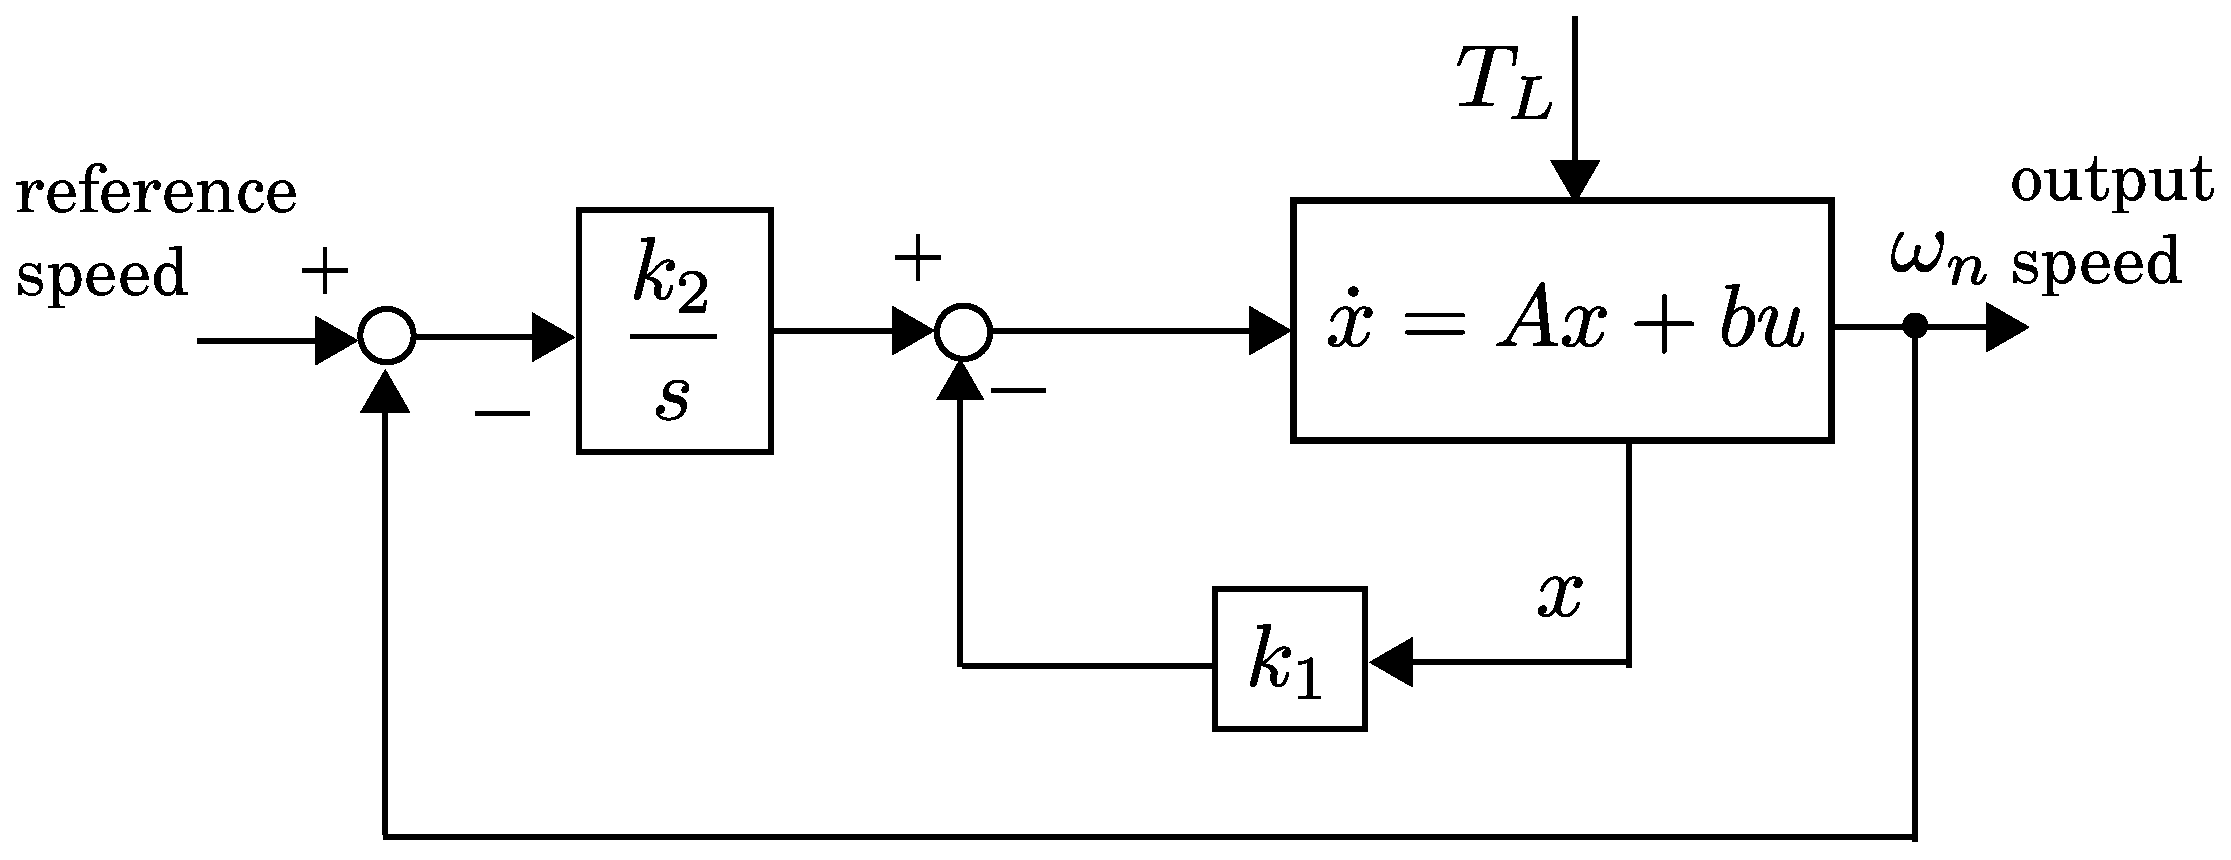
\includegraphics[width = 150mm]{fig/LQI_model.eps}
 \end{center}
 \caption{LQI制御系}
 \label{fig:LQI_model}
\end{figure}
%
この制御法を利用するため,
はじめにDCモータの支配方程式を導出する.DCモータの支配方程式は
%
\begin{eqnarray}
 \begin{cases}
  v = K_{E}\omega_m + R_{a}i_{a} + L_{a} \frac{di_a}{dt} & \\
  K_{T}i_a = J \frac{d\omega_m}{dt} + T_{L}
 \end{cases}
\end{eqnarray}
%
となる.$v$はDCモータへの入力電圧である.
ここで$u=v$,$x=(i_a  \ \omega_m)^t \ $(ただし,$i_a$は電機子電流,
$\omega_m$は出力速度)とおき,$T_L=0$として,DCモータの状態方程式を求めると,
\begin{equation}
 \frac{dx}{dt} =
  \begin{pmatrix}
   - \frac{R_a}{L_a} & -\frac{K_E}{L_a} \\
   \frac{K_T}{J} & 0
  \end{pmatrix}
  x +
\begin{pmatrix}
 \frac{1}{L_a} \\
 0
\end{pmatrix}
u = Ax + bu
\end{equation}
となる.係数行列$A,b$は
%
\begin{eqnarray}
 \begin{cases}
A=
  \begin{pmatrix}
   - \frac{R_a}{L_a} & -\frac{K_E}{L_a} \\
   \frac{K_T}{J} & 0
  \end{pmatrix}
  =
  \begin{pmatrix}
   -50  & -2833.3 \\
   0.85 & 0
  \end{pmatrix}
  & \\
  b =
  \begin{pmatrix}
   333.3 \\
   0
  \end{pmatrix}
 \end{cases}
\end{eqnarray}
%
となる.ここで拡大系の状態方程式は,
%
\begin{equation}
 \delta \dot{x}_e = A_{e}\delta x_e + b_e w
\end{equation}
%
となり,係数行列は,
%
\begin{eqnarray}
 \begin{cases}
A_e=
  \begin{pmatrix}
   A & b \\
   0 & 0
  \end{pmatrix}
  =
  \begin{pmatrix}
   -50  & -2833.3 & 333.3 \\
   0.85 & 0       & 0   \\
   0    &  0      &   0\\
  \end{pmatrix}
  & \\
  b_e =
  \begin{pmatrix}
  \ 0 \ \\
  \ 0 \ \\
  \ 1 \
  \end{pmatrix}
 \end{cases}
\end{eqnarray}
%
と求めらる.評価関数は
%
\begin{equation}
J_e = \int_{0}^{\infty} (\delta x_e^{T}Q_{e}\delta x_e + r_e w^2 ) dt 
\label{eq:hyouka}
\end{equation}
%
\begin{equation}
 Q_e = c_e^Tc_e = (c \ \ 0)^t(c \ \ 0) =
\begin{pmatrix}
 0 \\
 1 \\
 0
\end{pmatrix}
%
\begin{pmatrix}
 0 & 0 & 1
\end{pmatrix}
%
=
%
\begin{pmatrix}
 0 & 0 & 0 \\
 0 & 1 & 0 \\
 0 & 0 & 0
\end{pmatrix}
\end{equation}
%
である.重み$r_e$を$r_e=0.001$とし,LQ問題を計算するとフィードバックゲイ
ン$k_e$は
%
\begin{equation}
 k_e = b_e^{T}P_e/r_e
\end{equation}
%
で求められる.ただし,行列$P_e$はリッカチ方程式
%
\begin{equation}
 A_e^{T}P_e + P_e A_e + Q_e - P_e b_e b_e^T P_e /r_e = 0
\end{equation}
%
の正定対称解である.これを解くと,
%
\begin{equation}
 P_e =
  \begin{pmatrix}
   0      & 0.0002 & 0 \\
   0.0002 & 0.0204 & 0.0001 \\
   0      & 0.0001 & 0.0037
  \end{pmatrix}
\end{equation}
%
を得る.(12)式に代入すれば,
%
\begin{equation}
k_e =
  \begin{pmatrix}
   0 & 0.1 & 3.7
  \end{pmatrix}
\end{equation}
%
となる.以上より,サーボ系のゲインとして,
%
\begin{equation}
 \begin{pmatrix}
  k_1 & k_2
 \end{pmatrix}
 =
 \begin{pmatrix}
  0.011 & 0.653  & 31.55
 \end{pmatrix}
\end{equation}
%
を得る.また,重み$r_e$を$r_e=1$としたとき,同様に計算すると,
%
\begin{eqnarray}
 \begin{cases}
P_e=
  \begin{pmatrix}
   0      & 0.0002 & 0 \\
   0.0002 & 0.0204 & 0 \\
   0      &   0    & 0.1176 
 \end{pmatrix}
  \\
k_e=
\begin{pmatrix}
 0 & 0 & 0.1176
\end{pmatrix}
\\
\begin{pmatrix}
 k_1 & k_2
\end{pmatrix}
=
\begin{pmatrix}
 0.0004 & 0.0208 & 0.9997 
\end{pmatrix}
 
\end{cases}
\end{eqnarray}
%
となりLQI速度制御系が設計できた.次節でこの制御系を用いて4象限運転を実現
する.

%%%%%%%%%%%%%%%%%%%%
\section{4象限運転}
%%%%%%%%%%%%%%%%%%%
4象限運転とは,1象限では正転運転,2象限では正転回生,3象限では逆転運転,
4象限では逆転回生を行う運転である.
ここで,前節で設計したLQI速度制御系にて4象限運転を実現したシミュレーション結果を
$r_e=0.001$のときを図\ref{fig:LQI_r0001}に,$r_e=1$のときを図
\ref{fig:LQI_r1}に示す.また,$r_e=0.05$のときを図\ref{fig:LQI_r005}に示
す.ただし,目標速度は運転開始と同時にDC
モータの基底速度である500[rpm],運転開始から20[s]後に0[rpm],運転開始か
ら40[s]後に-500[rpm],運転開始から60[s]後に0[rpm]と変化するように与えた.
%
\begin{figure}[htbp]
 \begin{center}
  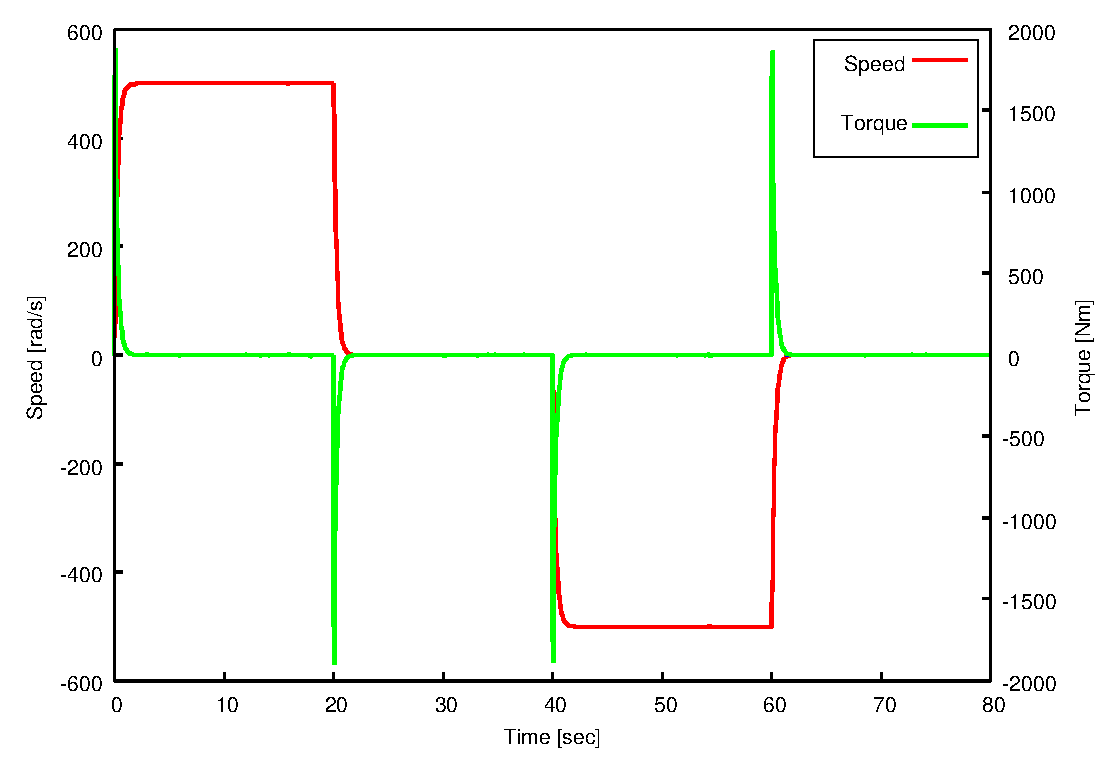
\includegraphics[width = 150mm]{fig/LQI_r0001.eps}
 \end{center}
 \caption{LQI制御によるDCモータの4象限運転のシミュレーション結果($r_e=0.001$)}
 \label{fig:LQI_r0001}
\end{figure}
%
%
\begin{figure}[htbp]
 \begin{center}
  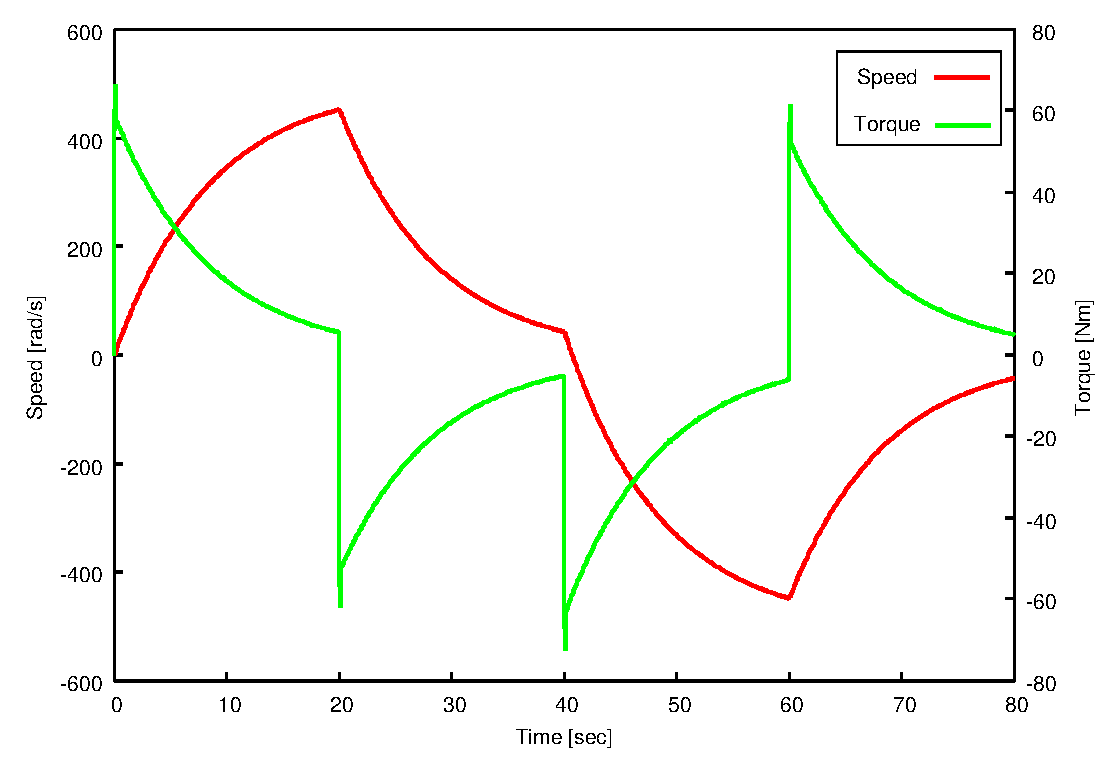
\includegraphics[width = 150mm]{fig/LQI_r1.eps}
 \end{center}
 \caption{LQI制御によるDCモータの4象限運転のシミュレーション結果($r_e=1$)}
 \label{fig:LQI_r1}
\end{figure}
%
%
\begin{figure}[htbp]
 \begin{center}
  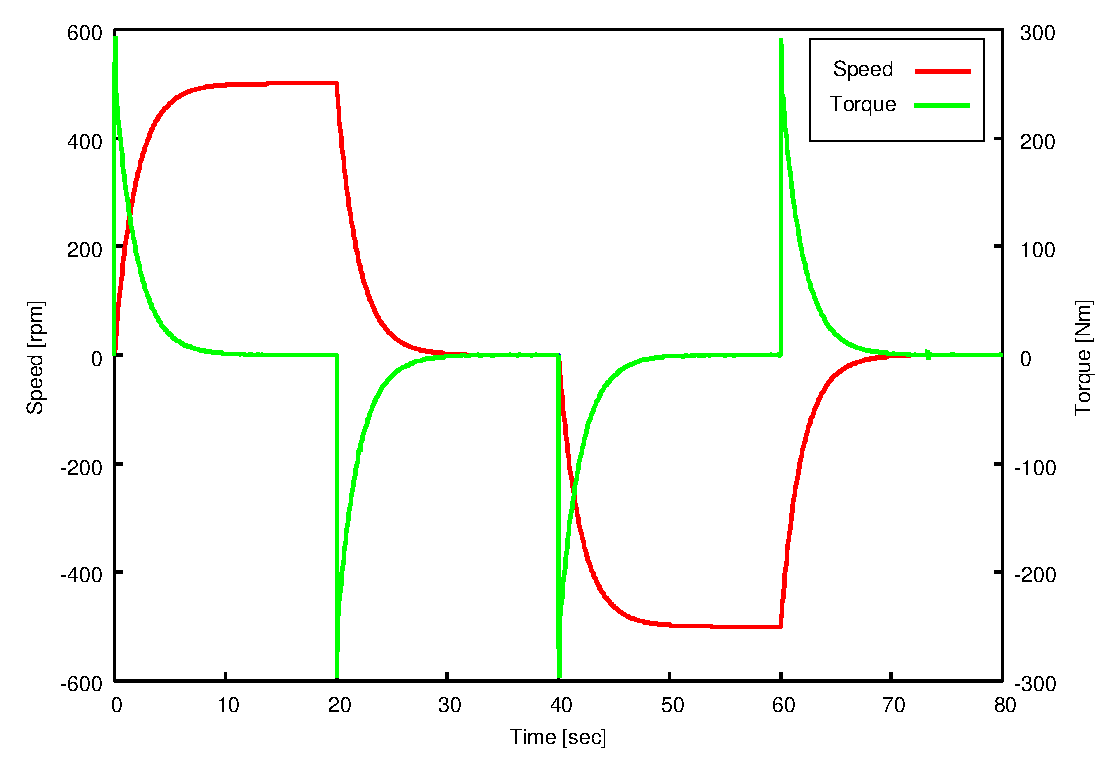
\includegraphics[width = 150mm]{fig/LQI_r005.eps}
 \end{center}
 \caption{LQI制御によるDCモータの4象限運転のシミュレーション結果($r_e=0.05$)}
 \label{fig:LQI_r005}
\end{figure}
%
%
図\ref{fig:LQI_r0001},\ref{fig:LQI_r1},\ref{fig:LQI_r005}を見ると,(\ref{eq:hyouka})式で示
した評価関数の重みを$r_e=1$としたときは$r_e=0.001$のときと比べて,応答が
遅く,出力トルクが小さいことがわかる.評価関数の重み$r_e$が大きいほど応
答が遅く,出力トルクが小さいのではないかと考えられる.速やかに目標速度に
到達させたい場合は評価関数を小さく設計すれば良いのではないかと考えられるが,小
さすぎると出力トルクが大きくなり,モータが破壊する可能性がある.よって評
価関数の重みを適切に選定する必要があると考えられる.

 
%
%%%%%%%%%%%%%%%%%%%%%%%%%%%%%%
%\section{カスケード速度制御系}
%%%%%%%%%%%%%%%%%%%%%%%%%%%%%%
%DCモータのカスケード制御系のブロック線図を図\ref{fig:cas2_model}に示す.
%ここで述べるカスケード制御系では一次ループとしての速度制御系の下位に二次
%ループとして電流制御系を構成し,制御量は速度と電流である.
%
%\begin{figure}[htbp]
 %\begin{center}
  %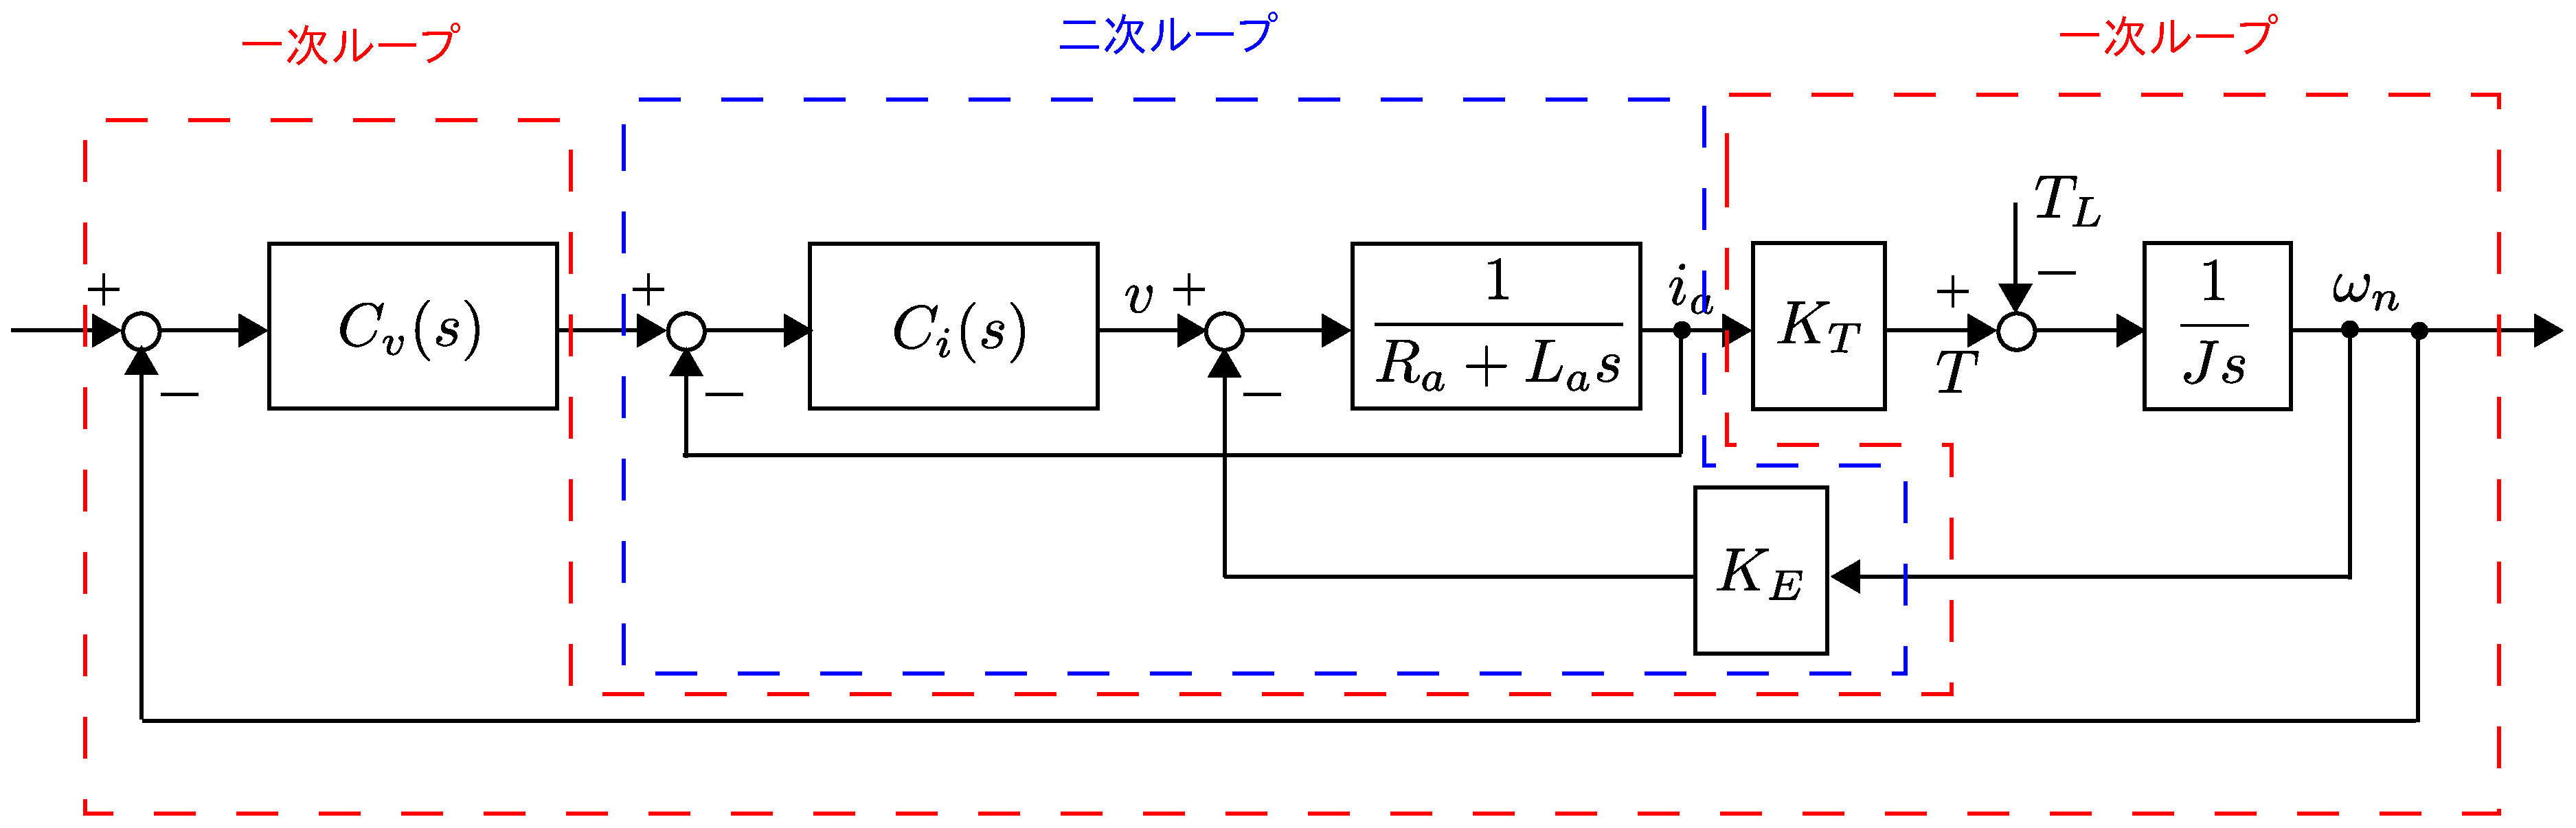
\includegraphics[width = 150mm]{fig/cas2_model.eps}
 %\end{center}
 %\caption{カスケード制御系のブロック線図}
 %\label{fig:cas2_model}
%\end{figure}
%
%速度制御系のゲイン交差周波数を100[rad/s],PIコントローラの折れ点周波数を
%20[rad/s]とおいてカスケード制御系を設計する.一次ループの開ループ伝達関
%数は,

%
\begin{thebibliography}{99}
\addcontentsline{toc}{section}{参考文献}

 \bibitem{denki} T.Sakamoto,
		 "Lecture Notes of Advanced Electrical Drive Control System", 2016.

 \bibitem{mecha} 坂本哲三, "電気機器の電気力学と制御", 森北出版, 2007.

\end{thebibliography}

\end{document}
